% vim:ts=4:sw=4
% Copyright (c) 2014 Casper Ti. Vector
% Public domain.

\chapter{随机脉冲仲裁PUF设计}\label{chap:rpapuf}
为了使 PUF 的安全性得到保障,统计分析和 NIST 测试通过是必要条件,尽可能提升模型复杂度也是必要条件。事实上,并不存在保证安全性的充分条件,因为总是有穷举的方法可以破解安全协议,而现有的攻击技术则是在一定时间成本下尽可能大的降低穷举复杂度。所以安全的攻和防是彼此的经济博弈,只有通过不断提升安全协议复杂度,同时又不增加系统开销,才能保证在相同经济能力下的相对安全性。

\ref{subsec:xormethod}节指出,多个 PUF 相异或可以提升总体模型的复杂度,将原N位 PUF 从 $ O(mn) $ 提升到 $ O(m'n^l) $, $ l $ 是异或输入个数。按现有的机器学习算法,当维度增加,训练集数量m也要增加才能保证训练效果,其不一定是线性关系,但总有 $ m'>m $,故异或可以呈指数幂增加攻击者成本开销,而自身代价则是线性地增加面积开销。文献\parencite{mahmoud2013combined}用 SVM 算法分析了现有的 PUF 和异或之后的 PUF 学习时间成本,如表\ref{tab:svm_learning_time}所示。

可以看出想要得到良好的效果,至少需要4个以上的 PUF 异或,从面积上来说,是一个不小的开销。本文的第二个设计 Pulse-based Arbiter PUF(PAPUF) 从减小面积的角度出发,达到在相同复杂度下,减小一半面积开销。

\begin{table}[htb]
\centering
\caption{仲裁PUF、XORPUF和Lightweight PUF学习时间开销统计}
\label{tab:svm_learning_time}
\begin{tabular}{|c|c|c|c|c|c|}
\hline
PUF Type                         & 激励位宽              & 预测率 & 输出异或个数 & 训练集CRP & 学习时间\\ 
\hline
仲裁型PUF                         & 128                  & 99\%  & -      & 5.5k   & 0.51s    \\ \hline
\multirow{6}{*}{XOR PUF}         & \multirow{3}{*}{64}  & 99\%  & 4      & 12k    & 3min42s  \\ \cline{3-6} 
                                 &                      & 99\%  & 5      & 80k    & 2h8min   \\ \cline{3-6} 
                                 &                      & 99\%  & 6      & 200k   & 31h1min  \\ \cline{2-6} 
                                 & \multirow{3}{*}{128} & 99\%  & 4      & 24k    & 2h52min  \\ \cline{3-6} 
                                 &                      & 99\%  & 5      & 500k   & 16h36min \\ \cline{3-6} 
                                 &                      & -     & 6      & -      & -        \\ \hline
\multirow{6}{*}{Lightweight PUF} & \multirow{3}{*}{64}  & 99\%  & 4      & 12k    & 1h28min  \\ \cline{3-6} 
                                 &                      & 99\%  & 5      & 300k   & 13h6min  \\ \cline{3-6} 
                                 &                      & -     & 6      & -      & -        \\ \cline{2-6} 
                                 & \multirow{3}{*}{128} & 99\%  & 4      & 500k   & 59min42s \\ \cline{3-6} 
                                 &                      & 99\%  & 5      & 1000k  & 267days  \\ \cline{3-6} 
                                 &                      & -     & 6      & -      & -        \\ \hline
\end{tabular}
\end{table}


\section{电路结构}\label{sec:rpa_scheme}
图\ref{fig:mux_logic}展示了仲裁型 PUF 一个交换器中 MUX 的逻辑级设计,在一个逻辑门中,对输出节点充电靠 PMOS 管,而 放电靠 NMOS 管,在工艺中 PMOS 和 NMOS 的掺杂是相互独立的,因此每个逻辑门充电和放电时间分别服从 $ N\sim(7.46\times 10^{-12}, 4.72\times 10^{-13}), N\sim(9.61\times 10^{-12}, 8.54\times 10^{-13}) $ , 的高斯分布。由此推出交换器对于上升沿信号的延迟和下降沿信号的延迟是不同的,故完整描述一个交换器需要8个变量(而非4个)。

\begin{figure}[htb]
\centering
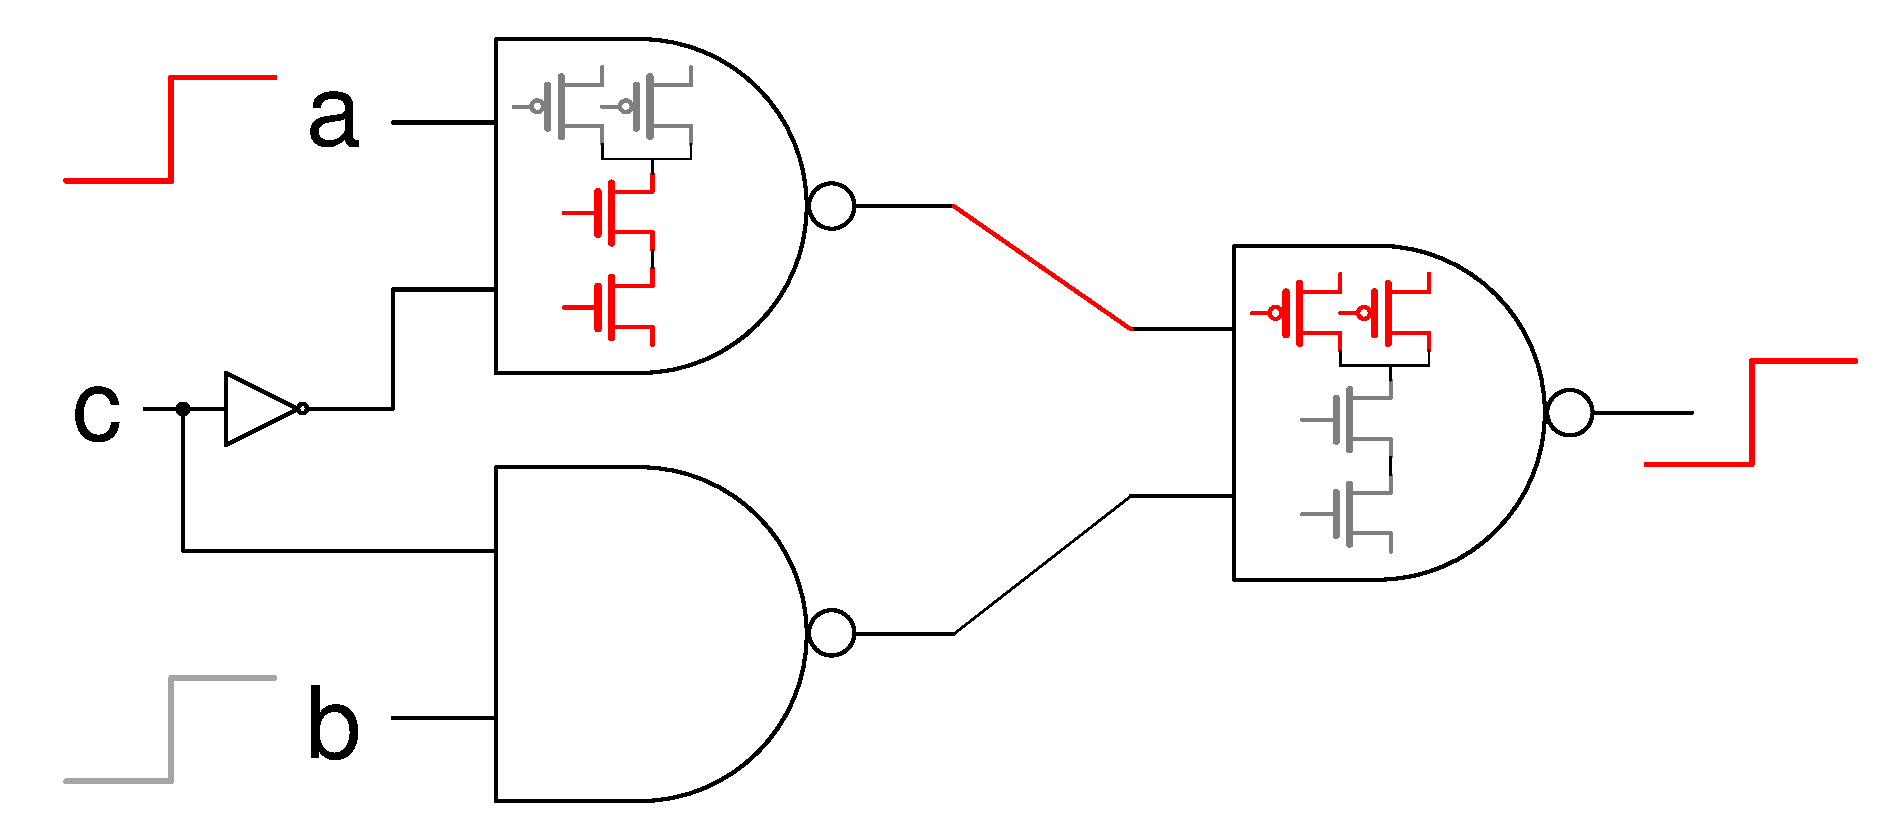
\includegraphics[width=.6\linewidth]{mux_logic_level}
\caption{交换器MUX设计电路图}
\label{fig:mux_logic}
\end{figure}

如图\ref{fig:papuf}所示,修改仲裁型 PUF 的输出,使最后一级交换器输出接入两个触发器 DFF1, DFF2,其中 DFF1 是正边沿锁存, DFF2 是负边沿锁存。复位之后,输入给入一个宽w的脉冲信号,其中上升沿会被 DFF1 采样,$ R_1=sgn(P'D_1 ) $,下降沿则被 DFF2 采样,$ R_2=sgn(P'D_2 ) $ 。输出 $ R=R_1\oplus R_2 $,由于参数 D1 与 D2 独立,所以输出响应R在$ n^2 $维度线性可分,与2个仲裁型 PUF 异或相当,但是面积减小了一半。

\begin{figure}[htb]
\centering
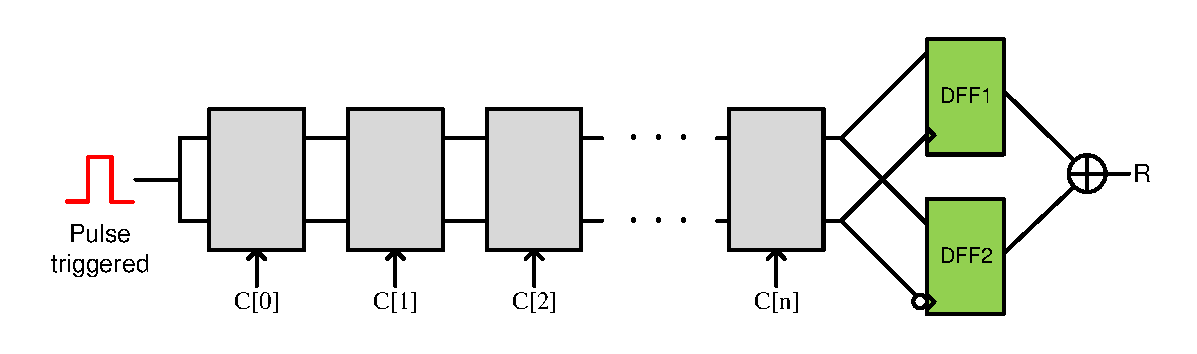
\includegraphics[width=\linewidth]{papuf}
\caption{PAPUF结构图}
\label{fig:papuf}
\end{figure}

下面考虑脉冲宽度w。在经过每一级交换器后,由于延迟时间的不等,w会发生变化,记 $ w_0 (n),w_1 (n) $ 为第n级交换器输出后顶/底两个节点的信号脉宽。
若w足够长,则能都正常通过N级交换器最后被触发器采样;倘若w足够小,那么当经过第i级交换器时,若上升沿延迟远远长于下降沿延迟,则 $ w(i+1)<0 $ (省略掉下标因为具体是哪个节点并不重要)。
这意味着第i级交换器并不会输出脉冲,将这种现象称为短脉冲的``消失''。
为了进一步增加抵抗建模攻击的能力,需要增加模型复杂度。
利用脉冲``消失''属性,令w恰好满足对所有激励有一定概率使得脉冲信号不会传递至寄存器,即在中途``消失''了。
对于消失的脉冲,两个寄存器都会采样出逻辑``0''(或者没有时钟信号,保持原值0)。

\begin{figure}[htb]
\centering
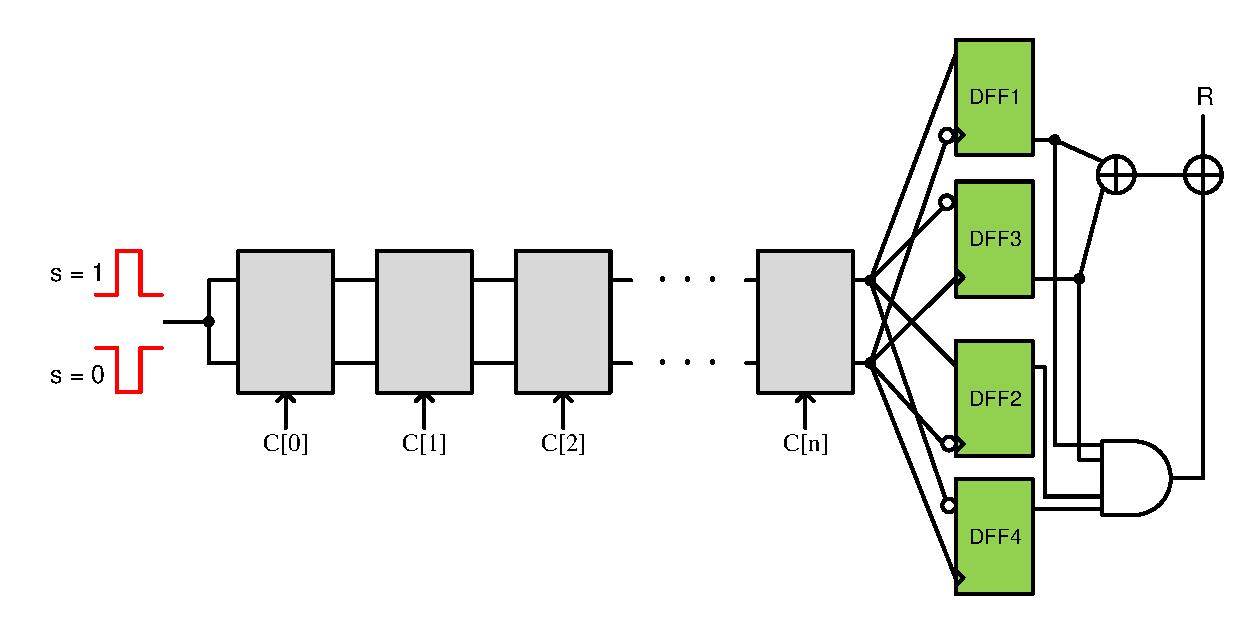
\includegraphics[width=\linewidth]{rpapuf}
\caption{改进的PAPUF结构图}
\label{fig:rpapuf}
\end{figure}

构建如图\ref{fig:rpapuf}所示的电路,输出由4个寄存器DFF1--DFF4组成,分别以正、负边沿采样两个节点。
复位时,先生成随机码s,若s为0,则寄存器复位为0,输入正脉冲$ {p}_0 $;若s为1,则寄存器复位为1,输入负脉冲$ {p}_1 $。
若脉冲信号正常传输至寄存器DFF1--DFF4,则 $ Q_1=r_1,~Q_2=\overline{r_1},~Q_3=r_2,~Q_4=\overline{r_2} $; 若脉冲信号消失,则有 $ Q_1=Q_2=Q_3=Q_4=s $。
输入采用 如下所述的策略:以50\%概率产生一个正脉冲,有50\%概率产生一个负脉冲, $ \mathrm{P}(p_0)=\mathrm{P}(p_1)=0.5  $。
这样,当脉冲正常传输时, DFF1--DFF4 寄存器采样到的值与正负脉冲无关,而当脉冲在中途消失时,则有以下几种情况:

\begin{itemize}
\item 正负脉冲均不能传递过去,则对于正脉冲,$ Q1=Q2=Q3=Q4=0 $;对于负脉冲$ Q1=Q2=Q3=Q4=1 $;
\item 正脉冲可以传递,负脉冲消失。则当s=1时,响应恒为1;
\item 负脉冲可以传递,正脉冲消失。则当s=0时,响应恒为0.
\end{itemize}
考虑整体情况,对于任意激励 $ C_i $,由于正负脉冲发生的概率定为50\%,所以总体响应理论分布仍然是50\%。真值表见表\ref{tab:true-table-rpa}。

\begin{table}[h!]
\centering
\caption{RPAPUF真值表}
\label{tab:true-table-rpa}
\begin{tabular}{c|cccc|c}
\hline
s & $ Q_1 $ & $ Q_2 $ & $ Q_3 $ & $ Q_4 $ & 备注 \\
\hline
x & 0 & 1 & 0 & 1 & 正常传递\\
x & 0 & 1 & 1 & 0 & 正常传递\\
x & 1 & 0 & 0 & 1 & 正常传递\\
x & 1 & 0 & 1 & 0 & 正常传递\\
1 & 1 & 1 & 1 & 1 & 负脉冲消失\\
0 & 0 & 0 & 0 & 0 & 正脉冲消失\\
\hline
\end{tabular}
\end{table}

与普通PUF不同,在具体求值时,需要重复激励K次,若K次结果恒定(或在考虑到噪声情况下大概率为某恒定值),则取本次 CRP;
反之,若K次结果为随机值,则抛弃此激励,取另一激励重复以上步骤。
那么对于 PUF 的使用者来说,代价是 CRP 空间减小了,且求值时间增加了K倍。
而对于攻击者来说,则不能用 XOR PUF 的模型来统一描述所有情况,且取等量训练集 CRP 耗费的时间增加为K倍。

\section{统计分析}\label{sec:rpa_stat}
PAPUF 的模型和统计分布与 XOR PUF 相同,具体参见\ref{sec:relatedwork}节相关内容。
对于改进后 PAPUF(随机 PAPUF,记为 RPAPUF )分析,设在所有 CRP 中,正脉冲消失的概率为$ p_p $,负脉冲消失的概率为$ p_n $, CRP 的总数是 $ M=2^N $。且:

\begin{equation}
R=Q_1\oplus Q_3\oplus (Q_1\cdot Q_2\cdot Q_3\cdot Q_4)
\end{equation}

假设一种理想模型,即在 PAPUF 的 CRP 中``1''严格地占50\%;而在 RPAPUF 中,随机码 s 严格遵循均匀分布。
则在 RPAPUF 中将整个 CRP 集合分为3个子集,记作 $ {P_{0}, P_{1}, P_{2} $ ,分别表示脉冲信号都完整传递的 CRP 集合、有且仅有一种脉冲信号完整传递的 CRP 集合和两种脉冲信号全都消失的 CRP 集合。
对于 $ P_0 $, 有响应 $ R(i) = f_{xor}(C_i) $, $ f_{xor} $ 即 XOR PUF 的表征模型,具体参见\ref{subsec:xormethod}节的内容。
而对于 $ P_2 $, 有 $ R(i) = s $。
最后对于 $ P_1 $,若负脉冲没有传递到寄存器,则 $ R(i)= f_{xor}(C_i)+s $ ; 若正脉冲没有传递到寄存器,则 $ R(i)=f_{xor}(C_i)\cdot s $ 。
根据前面的假设,$ P_0 $ 在全集应占比 $ (1-p_p)(1-p_n) $ , $ P(P_1)=p_p+p_n-2p_pp_n $, $ P(P_2)=p_pp_n $。

假设攻击者没有经过多次采样而直接用 XOR PUF 模型进行预测,则在训练集CRP中存在若干``随机点''。
易知,若随机点过少,则不会对建模造成影响,因为SVM学习过程中有``惩罚系数''可以过滤掉这部分数据,但是当随机点在训练CRP中占比上升,则训练效果会直线下降。
图\ref{fig:xor-svm-random}显示了用10000个CRP作为训练集学习 XOR PUF 模型参数,当随机点占比变化时预测率的变化。

\begin{figure}[htb!]
\centering
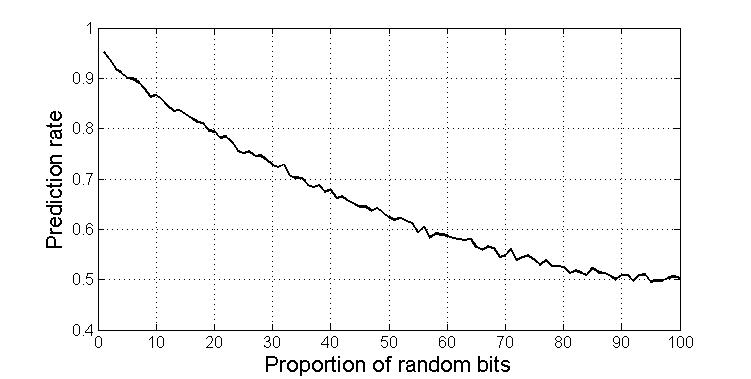
\includegraphics[width=.8\linewidth]{xorpuf_svm_randompoints}
\caption{XOR PUF预测率与训练集随机点占比的关系}
\label{fig:xor-svm-random}
\end{figure}

下面考虑对 RPAPUF 的建模攻击。
首先,攻击者必须对每一个激励重复若干次,以抛弃掉脉冲``消失''的(或``随机''的) CRP,因为消失的响应不满足 XOR PUF 模型;其次,对于剩下的 CRP ,有一部分属于 $ P_1 $ 。 即虽然该部分 CRP 某些脉冲激励``消失''了,但响应输出与随机码 s 无关,因此无法被攻击者过滤掉,所以攻击者只有50\%的概率判断此 CRP 的脉冲是否消失。
对于正常情况,响应仍满足 XOR PUF 的模型,但对于消失脉冲,第i级以后的的交换器不再产生作用,因此攻击者需要遍历N个节点,以寻找在哪个节点脉冲消失了。故建模的复杂度远远超过 $ m\cdot n^2 $ 量级\footnote{$ m $是SVM训练集中CRP个数,$ n^2 $是最小线性可分维度。}。

综上,使用者以 CRP 缩小的代价换取复杂度的显著提升,图\ref{fig:xor-svm-random}显示,为了达到最大效果, 应调节脉宽宽度使得 CRP 全集中至少50\%的脉冲不能传递到寄存器。
故 RPAPUF 以多次求值和 CRP 缩小一半的单价提升了建模复杂度。


\section{仿真验证}\label{sec:rpa_simu}
与\ref{chap:buildingmodel},\ref{chap:dbrpuf}章相同,采用 HSPICE 与 Matlab 结合的方式仿真。
不过由于本结构 RPAPUF 建模困难,采用迭代算法算出每一级交换器的输出延时,并判断该节点脉冲信号是否消失——若消失,则退出迭代,输出寄存器赋值``0''或``1'';否则迭代到N并计算延迟差。

脉冲宽度会显著影响结果,我们取宽度 $ w/d={1,10,100,1000} $,即倍率指数增长,1倍意味着根本没有任何脉冲信号能传递到寄存器,采样的值永远随着脉冲变化,因此响应因为随机值;1000倍意味着所有脉冲都能传递到寄存器,与正负脉冲无关,所以退化到PA PUF 。根据不同的脉宽,统计100个 PUF,每个 PUF 随机输入4096个32位激励得到的响应。图\ref{fig:rpa-single-rand}展示了 RPAPUF 的单次采样下随机性分布示意图。

\begin{figure}[htb!]
\centering
\subfloat[W/D = 1]{
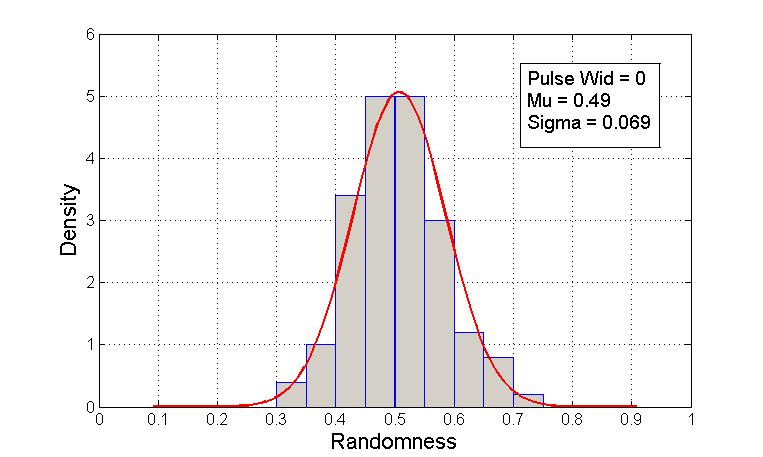
\includegraphics[width=.5\linewidth]{rpapuf_rand_pw0}
}
\subfloat[W/D = 10]{
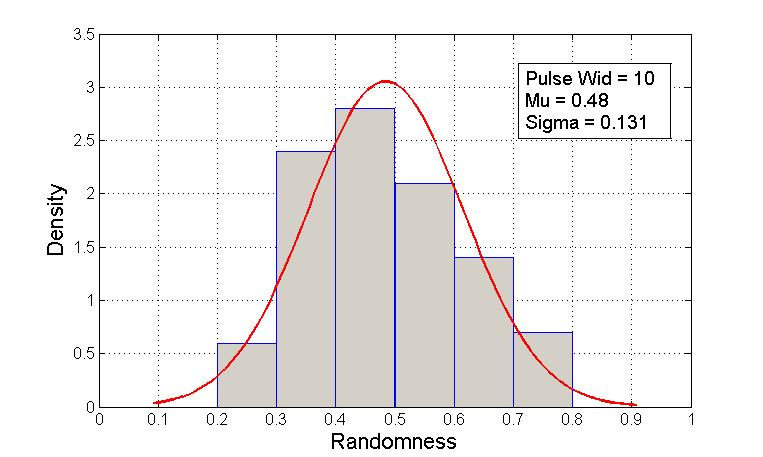
\includegraphics[width=.5\linewidth]{rpapuf_rand_pw10}
}\\
\subfloat[W/D = 100]{
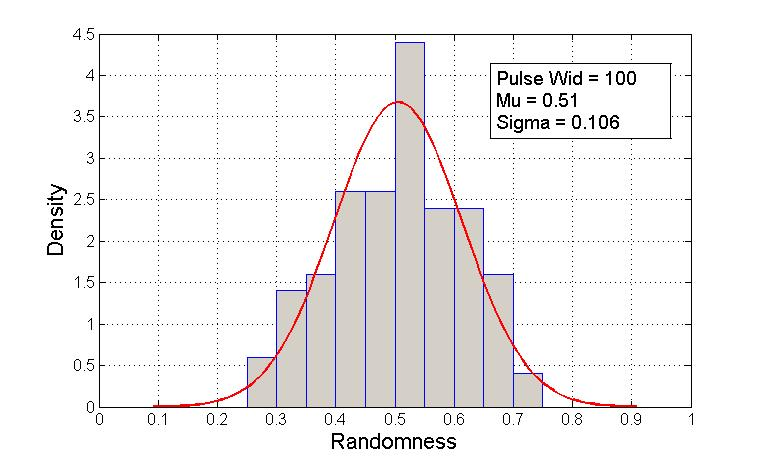
\includegraphics[width=.5\linewidth]{rpapuf_rand_pw100}
}
\subfloat[W/D = 1000]{
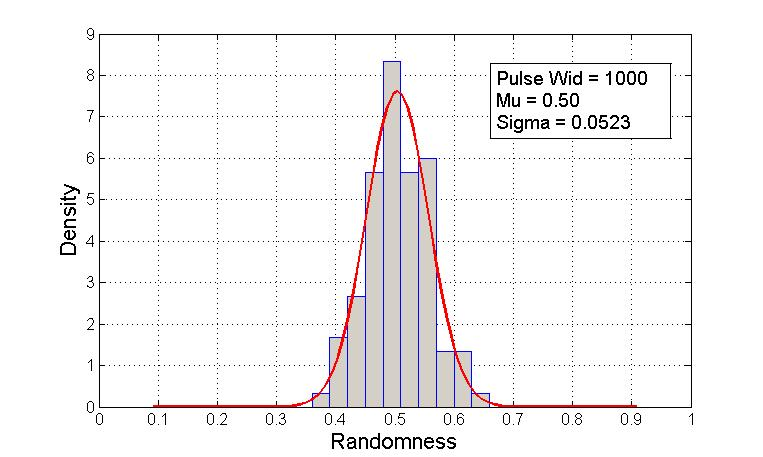
\includegraphics[width=.5\linewidth]{rpapuf_rand_pw1000}
}
\caption{RPAPUF单次采样随机性分布柱状图}
\label{fig:rpa-single-rand}
\end{figure}

可以看出,随着w的变化,R的输出分布变化并不明显,说明宏观上难以分辨出脉冲信号是否传递到寄存器,若采用 XOR PUF 建模方法,则会严重受到随机脉冲的干扰。
图\ref{fig:rpa-k100-rand}是脉宽延时比设为100时经过100次采样过滤后的随机性分布。

\begin{figure}[htb!]
\centering
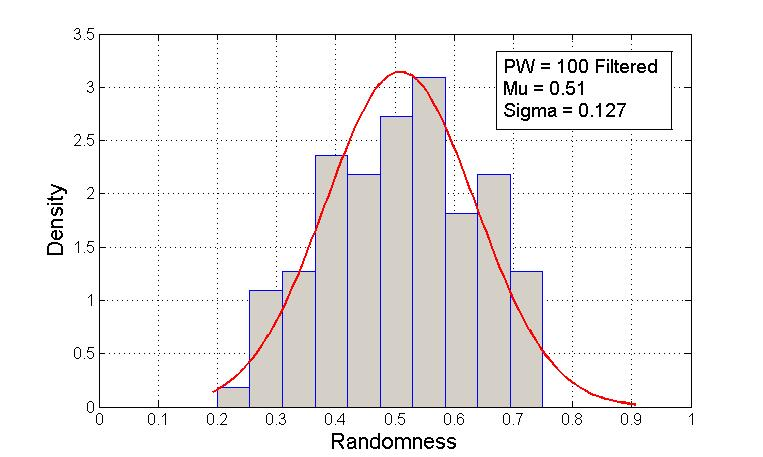
\includegraphics[width=.8\linewidth]{rpapuf_rand_pw100_filter}
\caption{RPAPUF 100次采样过滤随机响应后的随机性分布}
\label{fig:rpa-k100-rand}
\end{figure}

我们尝试用 XOR PUF 的模型对 RPAPUF 进行建模攻击, 图\ref{fig:rpa-svm}展示了对 32 位 RPAPUF 的攻击结果,虚线为训练集 CRP 单次采样的结果,即不分辨``消失''脉冲;
实线为训练集 CRP 多次采样,抛弃随机变化的点,能够过滤到部分``消失''脉冲。
图\ref{fig:rpa-svm-devices}显示训练集CRP在10000个的情况下,不同PUF在SVM建模后的预测率,横轴对应的是不同的器件。
可以看出无论响应过滤与否均不能达到很好的效果, 即使过滤掉部分随机 CRP,预测率并不会随着训练集 CRP 增加而增多。
同时也看出,随着片间分布变化,在某些情况下,恰好随机脉冲作用不明显(比如几乎没有消失,或者消失掉的部分恰好符合模型函数),使得有几个 PUF器件的点预测率非常高,这给我们留下了下一步的工作——分析随机脉冲在片内和片间的分布,尤其是脉冲宽度与工艺之间取何值最优。在现在的工作中囿于计算能力,不能再进一步分析。

\begin{figure}[htb!]
\centering
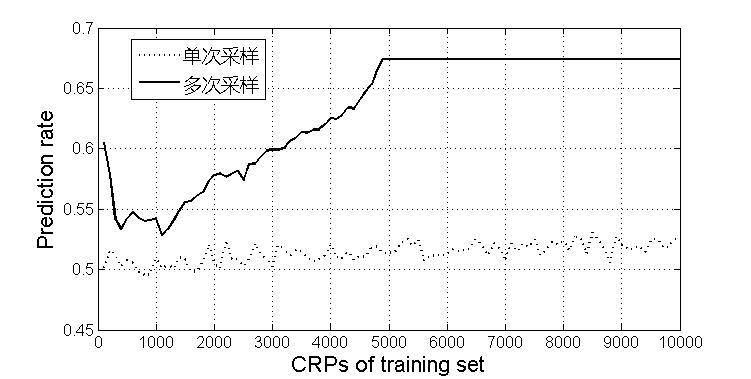
\includegraphics[width=.8\linewidth]{rpa_svm_single}
\caption{RPAPUF SVM预测结果(单一器件)}
\label{fig:rpa-svm}
\end{figure}

\begin{figure}[htb!]
\centering
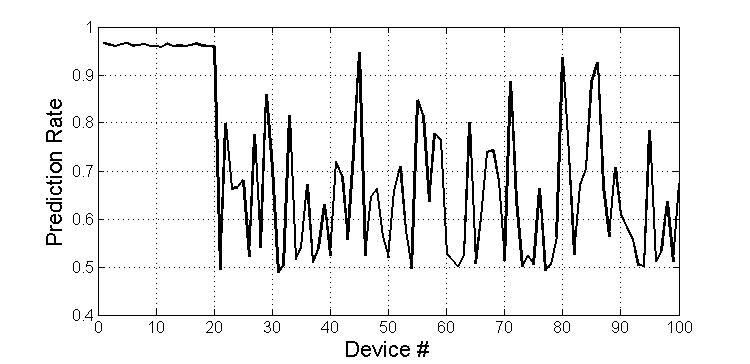
\includegraphics[width=.8\linewidth]{rpa_svm_devices}
\caption{RPAPUF SVM预测结果(跨器件统计)}
\label{fig:rpa-svm-devices}
\end{figure}

\section{几种PUF结构横向对比暨本章小结}\label{sec:rpa_summary}
本节提出并分析了新型随机脉冲型 PUF。
至此,本文一共分析了5种不同的 PUF 结构,表\ref{tab:puf_cmp}对其基本信息做了整理,表\ref{tab:puf_nist}展示了所有 PUF 的 NIST 测试结果\footnote{每PUF测试100个器件仿真结果取32768比特响应}。
在图\ref{fig:pufs_rand}中绘出所有 PUF 的随机性分布拟合曲线,图\ref{fig:pufs_uniq}则绘出了独特性的拟合曲线。

\begin{table}[htb]
\centering
\caption{PUF特征对比}\label{tab:puf_cmp}
\begin{tabular}{cccc}
\hline
PUF			& CRP空间	   & 最小线性可分空间维度 & 面积开销\\
\hline
Arbiter PUF & $ 2^N $ 	& N & N个交换器 			\\
2-XOR PUF	& $ 2^N $ 	& $ N^2 $ & 2N个交换器	    \\
BRPUF		& $ 2^N $ 	& N & 2N个与非门和多路器 	 \\
4-DBRPUF	& $ 2^N $ 	& N & N+4个交换器和8个与非门 \\
RPAPUF		& $ 2^{N-1} $ & - & N个交换器 		   \\
\hline
\end{tabular}
\end{table}

\begin{table}[htb]
\centering
\caption{PUF NIST测试通过率}
\label{tab:puf_nist}
\begin{tabular}{cccccc}
\hline
NIST Test & Arbiter & 2-XOR & BRPUF & 4-DBRPUF & RPAPUF \\
\hline
Frequency & & & & &\\
Block Frequency & & & & &\\
Cumulative Sums & & & & &\\
Runs & & & & &\\
Longest Run & & & & &\\
Rank & & & & &\\
FFT & & & & &\\
Universal & & & & &\\
Approximate Entropy & & & & &\\
Serial & & & & &\\
Linear Complexity & & & & &\\
Random Excursions & & & & &\\
Random Excursions Variant & & & & &\\
Overlapping Template & & & & &\\
Nonperiodic Template & & & & &\\
\hline
\end{tabular}
\end{table}

\begin{figure}[htb]
\centering
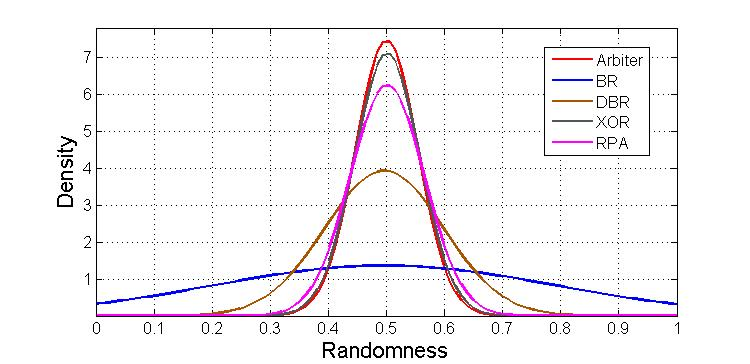
\includegraphics[width=.8\linewidth]{rand_5pufs}
\caption{PUF随机性分布拟合曲线}
\label{fig:pufs_rand}
\end{figure}

\begin{figure}[htb]
\centering
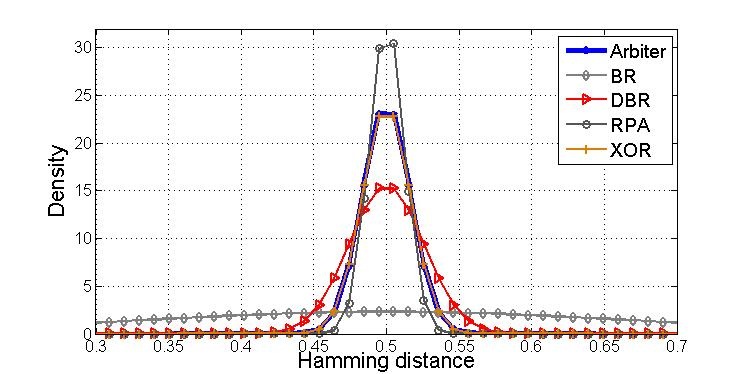
\includegraphics[width=.8\linewidth]{uniq_5pufs}
\caption{PUF独特性分布拟合曲线}
\label{fig:pufs_uniq}
\end{figure}

可以看出,综合比较, DBRPUF 优于 BRPUF,但两者相比于传统仲裁型 PUF 在随机性上仍不足。改进后的 XOR PUF 和 RPAPUF 则在统计结果上优于传统仲裁型 PUF,而本文所提出的 RPAPUF 在面积上优于 XOR PUF。最后,图\ref{fig:svm_all}给出了 SVM 机器学习结果,根据我们的建模,仲裁型 PUF 和 BRPUF 能够用1000个训练集达到95\%以上的预测成功率,而 XOR PUF 则需要超过5000个训练集,耗费数倍时间才能达到95\%的成功率。对于 RPAPUF,因为建模困难,我们用 XOR PUF 的模型进行学习,可以看出直接学习的成功率仅有50\%,根随机猜测一样,而经过多次采样过滤后的预测成功率最高也仅达到67\%,在有限的时间内并不能更进一步提升其预测率,故安全性上评价总结见表\ref{tab:puf_cmp}。

\begin{figure}[htb!]
\centering
%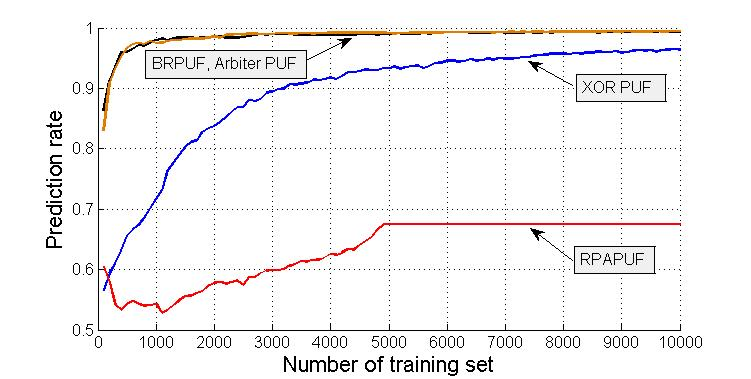
\includegraphics[width=.8\linewidth]{svm_all}
\caption{不同PUF SVM预测率对比}
\label{fig:svm_all}
\end{figure}
